\subsection{Round 1 Solutions}\label{S::2024-S-1}

\begin{resources}
    Review by \resit{https://www.youtube.com/watch?v=bL4s-qHweKg}{Way Tan}
\end{resources}

\begin{question}[D]\label{A::2024-S-1-1}
    Find the largest positive integer $A$ such that $2^x + \dfrac{2025}{2^x} - A > 0$ for all real numbers $x$

    \begin{tasks}(5)
        \task 59
        \task 69
        \task 79
        \task 89
        \task 99
    \end{tasks}
\end{question}
\begin{solution*}
    Multiplying through by $2^x$ (which does not affect the inequality since $2^x > 0$), we get a quadratic in $2^x$: \[\bp{2^x}^2 - A \cdot 2^x + 2025 > 0.\] The discriminant of this quadratic must be less than 0, hence \[A^2 - 4 \cdot 2025 < 0.\] Solving, we get $A < 50$, whence $\max A = 49$.
\end{solution*}

\begin{question}[B]\label{A::2024-S-1-2}
    If $x = \dfrac{1}{\log_{\frac{2024}{2023}} 7} + \dfrac{1}{\log_{\frac{2023}{2022}} 7} + \dfrac{1}{\log_{\frac{2022}{2021}} 7}$, find $7^x$.

    \begin{tasks}(5)
        \task $\dfrac{2021}{2024}$
        \task $\dfrac{2024}{2021}$
        \task $\dfrac{2022}{2024}$
        \task $\dfrac{2024}{2022}$
        \task $2024$
    \end{tasks}
\end{question}
\begin{solution*}
    Recall the change of base formula for logarithms: $\log_b a = \frac{\ln a}{\ln b}$. We hence get \[x = \frac{\ln \frac{2024}{2023}}{\ln 7} + \frac{\ln \frac{2023}{2022}}{\ln 7} + \frac{\ln \frac{2022}{2021}}{\ln 7} = \frac{\ln \frac{2024}{2021}}{\ln 7} = \log_7 \frac{2024}{2021},\] where we used the property $\log a + \log b = \log ab$ in the intermediate step. Thus, $7^x = \frac{2024}{2021}$.
\end{solution*}

\clearpage
\begin{question}[D]\label{A::2024-S-1-3}
    Simplify $\dfrac{2024}{\sqrt{4 + \sqrt{12}}} + \dfrac{2024}{\sqrt{4 - \sqrt{12}}}$.

    \begin{tasks}(5)
        \task 1012
        \task $1012\sqrt3$
        \task 2024
        \task $2024\sqrt3$
        \task! $1012 + 1012\sqrt3$
    \end{tasks}
\end{question}
\begin{solution*}
    Observe that $4 \pm \sqrt{12} = \sqrt{3}^2 \pm 2\sqrt{3} + 1 = \bp{\sqrt{3} \pm 1}^2$. Hence, we see that \[\frac{2024}{\sqrt{4 + \sqrt{12}}} + \dfrac{2024}{\sqrt{4 - \sqrt{12}}} = 2024 \bp{\frac1{\sqrt{3} + 1} + \frac1{\sqrt3 - 1}} = 2024\sqrt{3}.\]
\end{solution*}

\begin{question}[A]\label{A::2024-S-1-4}
    Suppose $x^{1/3} + 12 = y^{1/3}$ for some real numbers $x$ and $y$. Find the minimum possible value of $y-x$.

    \begin{tasks}(5)
        \task 432
        \task 532
        \task 632
        \task 732
        \task! None of the above
    \end{tasks}
\end{question}
\begin{solution}
    By the difference of cubes identity, one has \[y - x = \bp{y^{1/3} - x^{1/3}}\bp{y^{2/3} + y^{1/3}x^{1/3} + x^{2/3}} = 12\bp{y^{2/3} + y^{1/3}x^{1/3} + x^{2/3}}.\] Substituting $y^{1/3} = x^{1/3} + 12$, we see that \[y^{2/3} + y^{1/3}x^{1/3} + x^{2/3} = 3x^{2/3} + 36x^{1/3} + 144 = 3\bp{x^{1/3} + 6}^2 + 36.\] Hence, $y - x \geq 12 \cdot 36 = 432$, with equality when $x^{1/3} = -6$.
\end{solution}
\begin{solution}[Abusing symmetry]
    Let $x_\ast = -x$. We wish to find the minimum value of $x_\ast + y$ subject to $x_\ast^{1/3} + y^{1/3} = 12$. By symmetry, this occurs when $x_\ast^{1/3} = y^{1/3} = 6$, thus $\min x_\ast + y = 6^3 + 6^3 = 432$.
\end{solution}

\begin{question}[D]\label{A::2024-S-1-5}
    Find the largest possible value of $\dfrac{\sqrt2 \cos{2x}}{\sin{x} + \cos{x}}$.

    \begin{tasks}(5)
        \task $\dfrac12$
        \task 1
        \task $\dfrac32$
        \task 2
        \task $\dfrac52$
    \end{tasks}
\end{question}
\begin{solution*}
    Note that $\cos{2x} = \cos^2 x - \sin^2 x = (\cos x + \sin x)(\cos x - \sin x)$. Hence, \[\dfrac{\sqrt2 \cos{2x}}{\sin{x} + \cos{x}} = \sqrt{2} (\cos x - \sin x) = \sqrt2 \cdot \sqrt2 \cos{x - \frac{\pi}4},\] where we used the R-formula in the last step. Thus, the largest possible value is clearly 2.
\end{solution*}

\begin{question}[64]\label{A::2024-S-1-6}
    If $\sqrt{x + \sqrt{x}} + \sqrt{x - \sqrt{x}} = 4$, find the value of $15x$.
\end{question}
\begin{solution*}
    Squaring and simplifying, we get $\sqrt{x^2 - x} = 8 - x$. Squaring again, we get $x^2 - x = 64 - 16x + x^2$, whence $15x = 64$.
\end{solution*}

\begin{question}[242]\label{A::2024-S-1-7}
    Find the smallest positive integer $K$ such that \[x^2 - 200x + y^2 = 0 \text{ and } x + y \leq K.\]
\end{question}
\begin{solution*}
    Completing the square on the first equation, we clearly get the equation of a circle with centre $(100, 0)$ and radius 100: \[(x - 100)^2 + y^2 = 100^2.\] From the second equation, we have $y \leq K - x$. Since we are interested in the extreme values of $K$, we consider $y = K - x$. This is the equation of a line with gradient $-1$ and $y$-intercept $K$. Additionally, this line is tangent to the aforementioned circle, implying that the ``argument'' of the point of tangency to the centre of the circle is $45\deg$. Since $K > 0$, the point of tangency must be $(100 + 100\cos{45\deg}, 100\cos{45\deg}) = (100 + 50\sqrt2, 50\sqrt2)$. Using the point slope formula, we have \[y - 50\sqrt2 = -x + 100 + 50\sqrt2,\] whence the $y$-intercept is $100 + 100\sqrt{2} \approx 241.4$. Since $K$ is an integer, $\min K = 242$.
\end{solution*}

\begin{question}[506]\label{A::2024-S-1-8}
    Given that $\dfrac{\cos{x}}{\sin{3x}} - \dfrac{\sin{x}}{\cos{3x}} - 2 \cdot \dfrac{\sin{4x}}{\cos{6x}} = 2024$, find the value of $\dfrac{\cos{10x}}{\sin{12x}}$.
\end{question}
\begin{solution*}
    Observe that \[\frac{\cos x}{\sin 3x} - \frac{\sin x}{\cos 3x} = \frac{\cos x \cos 3x - \sin x \sin 3x}{\sin 3x \cos 3x} = \frac{2\cos 4x}{\sin 6x}.\] Plugging this into the given equation yields \[\frac{\cos 4x}{\sin 6x} - \dfrac{\sin 4x}{\cos 6x} = 1012.\] Playing the same game, we see that \[\frac{\cos 4x}{\sin 6x} - \dfrac{\sin 4x}{\cos 6x} = \frac{2\cos 10x}{\sin 12x}.\] Thus, \[\frac{\cos 10x}{\sin 12x} = \frac12 \cdot 1012 = 506.\]
\end{solution*}

\begin{question}[3]\label{A::2024-S-1-9}
    Find the smallest positive integer $k$ such that the coefficient of $x^k$ in the expansion of $\bp{5x^3 + \frac1{\sqrt{x}}}^{2024}$ is \textbf{not} zero.
\end{question}
\begin{solution*}
    By the binomial theorem, we have \[\bp{5x^3 + \frac1{\sqrt{x}}}^{2024} = \sum_{n = 1}^{2024} \binom{2024}{n} \bp{5x^3}^n \bp{x^{-\frac12}}^{2024-n} = \sum_{n = 1}^{2024} \binom{2024}{n} 5^n x^{\frac72 n - 1012}.\] Let $k = \frac72 n - 1012$. Since $k > 0$, we have $n \geq 290$. Since $\binom{2024}{290} 5^{290}$ is clearly non-zero, we have $\min k = \frac72 \cdot 290 - 1012 = 3$.
\end{solution*}

\begin{question}[2048]\label{A::2024-S-1-10}
    Let \[P = \bp{2024^2 + 1}\bp{2024^{2^2} + 1}\bp{2024^{2^3} + 1}\cdots\bp{2024^{2^{10}} + 1} \times 2025 + \dfrac1{2023}.\] Find the smallest positive integer $N$ such that $N > \log_{2024} P$.
\end{question}
\begin{solution*}
    Observe that \[P = \frac1{2023} + \prod_{k = 1}^{10} \bp{2024^{2^k} + 1}.\] Expanding out the product, it is easy to see that \[\prod_{k = 1}^{10} \bp{2024^{2^k} + 1} = \sum_{k = 0}^{2^{11} - 1} 2024^k,\] which evaluates to $\frac{2024^{2^{11}} - 1}{2024 - 1}$. Hence, \[P = \frac{2024^{2^{11}} - 1}{2023} + \frac1{2023} = \frac{2024^{2^{11}}}{2023} \implies \log_{2024} P = 2^{11} - \log_{2024} 2023.\] Clearly $\log_{2024} 2023 < 1$. Hence, $\min N = 2^{11} = 2048$.
\end{solution*}

\clearpage
\begin{question}[145]\label{A::2024-S-1-11}
    Let $\triangle ABC$ be a triangle with area 1000. Let $M$ and $N$ be points on $AB$ and $AC$ respectively such that \[AM : MB = 3 : 2 \text{ and } AN : NC = 7 : 3.\] Let $X$ and $Y$ be the midpoints of $BN$ and $CM$ respectively. Find the area of $\triangle AXY$.

    \begin{center}
        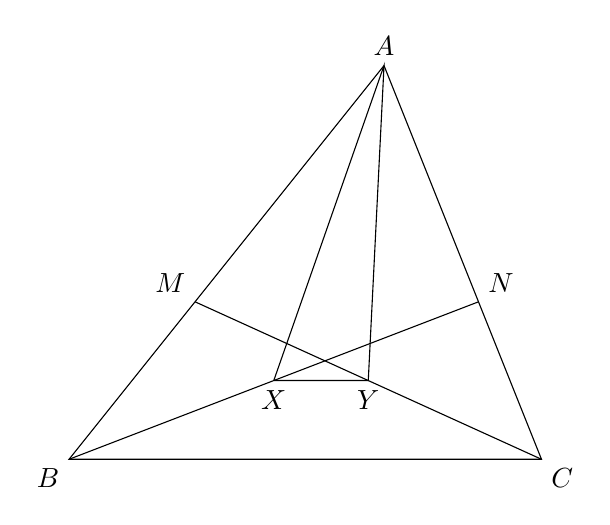
\begin{tikzpicture}
            \coordinate[label=above:$A$] (A) at (4, 5);
            \coordinate[label=below left:$B$] (B) at (0, 0);
            \coordinate[label=below right:$C$] (C) at (6, 0);
            \coordinate[label=above left:$M$] (M) at (1.6, 2);
            \coordinate[label=above right:$N$] (N) at (5.2, 2);
            \coordinate[label=below:$X$] (X) at (2.6, 1);
            \coordinate[label=below:$Y$] (Y) at (3.8, 1);

            \draw (A) -- (B) -- (C) -- (A);

            \draw (C) -- (M);
            \draw (B) -- (N);
            
            \draw (X) -- (A) -- (Y) -- (X);
        \end{tikzpicture}
    \end{center}
\end{question}
\begin{solution*}
    Observe that $\oa{AM} = \frac35 \oa{AB}$ and $\oa{AN} = \frac7{10} \oa{AC}$. By the midpoint theorem, it follows that \[\oa{AX} = \frac12 \bp{\frac35 \oa{AB} + \oa{AC}} \text{ and } \oa{AY} = \frac12 \bp{\frac7{10} \oa{AC} + \oa{AB}}.\] Thus, \[[AXY] = \frac12 \abs{\oa{AX} \crossp \oa{AY}} = \frac18 \abs{\bp{\frac35 \oa{AB} + \oa{AC}} \crossp \bp{\frac7{10} \oa{AC} + \oa{AB}}} = \frac{29}{200} \cdot \frac12 \abs{\oa{AB} \crossp \oa{AC}}.\] Since $[ABC] = \frac12 \abs{\oa{AB} \crossp \oa{AC}}$, we see that $[AXY] = \frac{29}{200} \cdot 1000 = 145$.
\end{solution*}

\begin{question}[8099]\label{A::2024-S-1-12}
    Find the largest positive integer $n \leq 10000$ such that $1 + 2024n^2$ is a perfect square.
\end{question}
\begin{solution*}
    Let $m$ be an integer such that $1 + 2024n^2 = m^2$. Then $m^2 - 2024n^2 = 1$. We thus have a Pell equation where $D = 2024$. The fundamental solution is clearly $m = 45$ and $n = 1$. The solutions $m_i$ and $n_i$ to the Pell equation are hence given by $m_i + \sqrt{2024}n_i = (45 + \sqrt{2024})^i$. When $i = 2$, we have \[(45 + \sqrt{2024})^2 = 4049 + 90\sqrt{2024} \implies n_2 = 90.\] When $i = 3$, we have \[(45 + \sqrt{2024})^3 = 364365 + 8099\sqrt{2024} \implies n_3 = 8099.\] Taking $i \geq 4$ will very clearly give us an $n$ greater than 10000. Thus, $\max n = 8099$.
\end{solution*}

\begin{question}[128]\label{A::2024-S-1-13}
    In a tetrahedron $SABC$, the faces $SBC$ and $ABC$ are perpendicular to each other. The angles $\angle ASB$, $\angle BSC$, $\angle ASC$ are all $60\deg$, and $SB = SC = 4$. Find the square of the volume of the tetrahedron.

    \begin{center}
        \begin{tikzpicture}[scale=0.8]
            \coordinate[label=left:$A$] (A) at (-1.5, 2);
            \coordinate[label=below:$B$] (B) at (0, 0);
            \coordinate[label=right:$C$] (C) at (5, 2);
            \coordinate[label=above:$S$] (S) at (3, 6);

            \draw (A) -- (B) -- (C) -- (S) --  (A);
            \draw[dashed] (A) -- (C);
            \draw (S) -- (B);
        \end{tikzpicture}
    \end{center}
\end{question}
\begin{solution*}
    Without loss of generality, let $SBC$ lie on the $x-z$ plane, and let $ABC$ lie on the $x-y$ plane. Since $\angle BSC = 60\deg$ and $SB = SC = 4$, it follows that $\triangle SBC$ is equilateral. Let $B(-2, 0, 0)$ and $C(2, 0, 0)$. Then $S(0, 0, 2\sqrt3)$. By symmetry, $A$ must lie on the $y$ axis. Hence, $A(0, a, 0)$ for some $a$ to be determined. Since $\angle ASB = 60\deg$, we have \[\oa{AS} \dotp \oa{BS} = AS \cdot BS \cdot \cos 60\deg \implies AS = 6.\] Let $O$ be the origin, which is also the midpoint of $BC$. Since $OA \perp BC$, by Pythagoras' theorem, we have \[OS^2 + OA^2 = AS^2 \implies a^2 = AS^2 - OS^2 = 24.\] Hence, $[ABC] = \frac12 BC \cdot OA = 4\sqrt6$. Thus, the volume of the tetrahedron is \[[SABC] = \frac13 \cdot [ABC] \cdot OS = 8\sqrt{2} \implies [SABC]^2 = 128.\]
\end{solution*}

\begin{question}[965]\label{A::2024-S-1-14}
    Let $a$, $b$, $c$ be the three real roots of the cubic equation \[2x^3 - 4x^2 - 21x - 8 = 0.\] Given that \[S = \frac1{ab + c -1} + \frac1{bc + a -1} + \frac1{ca + b - 1}\] is a rational number that can be expressed as a fraction in the lowest form $\frac{m}{n}$, find the value of $m^2 + n^2$.
\end{question}
\begin{solution*}
    By Vieta's formula, we have $abc = 4$ and $a + b + c = 2$. Hence, \[S = \frac{a}{a^2 - a + 4} + \frac{b}{b^2 - b + 4} + \frac{c}{c^2 - c + 4}.\] Now observe that \[2x^3 - 4x^2 - 21x - 8 = (x^2 - x + 4)(2x - 2) - 31 x.\] Since $a$, $b$, $c$ are roots of the cubic on the LHS, we get \[(a^2 - a + 4)(2a - 2) - 31a = 0 \implies \frac{a}{a^2 - a + 4} = \frac{2a - 2}{31},\] with identical expressions for $b$ and $c$. Substituting these expressions back into $S$, we have \[S = \frac{2a - 2}{31} + \frac{2b - 2}{31} + \frac{2c - 2}{31} = \frac{2(a+b+c) - 6}{31} = \frac{-2}{31}.\] Thus, $m^2 + n^2 = (-2)^2 + 31^2 = 965$.
\end{solution*}

\begin{question}[25]\label{A::2024-S-1-15}
    Consider the equation \[\frac{\sqrt3 - 1}{\sin x} + \frac{\sqrt3 + 1}{\cos x} = 4\sqrt2.\] For the range $0 < x < \pi/2$, the sum of the solutions of the equation can be expressed in the form $\frac{m\pi}{n}$, where $\frac{m}{n}$ is a fraction in the lowest form. Find $m + n$.
\end{question}
\begin{solution*}
    Observe that \[\frac{\sqrt3 - 1}{2} = \cos \frac\pi6 - \cos \frac\pi3 = 2\sin \frac\pi4 \sin \frac\pi{12} = \sqrt2 \sin \frac\pi{12}.\] Similarly, \[\frac{\sqrt3 + 1}{2} = \cos \frac\pi6 + \cos \frac\pi3 = 2\sin\frac\pi4 \cos\frac\pi{12} = \sqrt 2 \cos\frac\pi{12}.\] Our equation hence simplifies to \[\frac{\sin{\pi/12}}{\sin x} + \frac{\cos{\pi/12}}{\cos x} = 2 \implies \sin \frac\pi{12} \cos x + \cos x \sin \frac\pi{12} = 2\sin x \cos x,\] which very clearly gives us \[\sin{x + \frac\pi{12}} = \sin{2x}.\]

    \case{1} Suppose $2x = x + \frac\pi{12} + 2n\pi$, where $n$ is an integer. Then $x = \frac{24n + 1}{12}\pi$, whence the only solution in the given range is $x = \frac{\pi}{12}$.

    \case{2} Suppose $2x = (2n + 1)\pi - \bp{x + \frac\pi{12}}$, where $n$ is an integer. Then $x = \frac{24n + 11}{36} \pi$, whence the only solution in the given range is $x = \frac{11\pi}{36}$.

    Thus, the sum of solutions is $\frac{\pi}{12} + \frac{11\pi}{36} = \frac{7\pi}{18}$, whence $m + n = 25$.
\end{solution*}

\begin{question}[40]\label{A::2024-S-1-16}
    An engineer constructs a circle with centre $O$ and diameter $CD$ on level ground, and builds a vertical tower of height 20 at the centre. $B$ is another point on the circumference and $P$ is on $CD$ produced such that $PB$ is a secant line of the circle. Given that $PB = 33$, $PC = 77$ and $CD = 74$, find the minimum possible distance of any point on $PB$ to the top of the tower.

    \begin{center}
        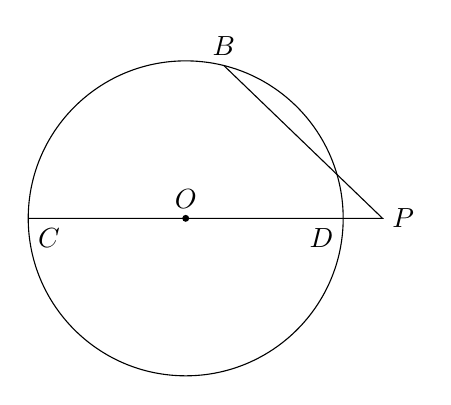
\begin{tikzpicture}[scale=0.5]
            \coordinate[label=above:$B$] (B) at (0.97, 3.88);
            \coordinate[label=right:$P$] (P) at (5, 0);
            \coordinate[label=below right:$C$] (C) at (-4, 0);
            \coordinate[label=below left:$D$] (D) at (4, 0);
            \coordinate[label=above:$O$] (O) at (0, 0);

            \draw (C) -- (P) -- (B);

            \draw (O) circle[radius=4];

            \fill (O) circle[radius=2.5pt];
        \end{tikzpicture}
    \end{center}
\end{question}
\begin{center}
    \begin{tikzpicture}[scale=0.5]
        \coordinate[label=above right:$A$] (A) at (3.84, 1.12);
        \coordinate[label=above:$B$] (B) at (0.97, 3.88);
        \coordinate[label=right:$P$] (P) at (5, 0);
        \coordinate[label=below right:$C$] (C) at (-4, 0);
        \coordinate[label=below left:$D$] (D) at (4, 0);
        \coordinate[label=left:$E$] (E) at (2.40, 2.498);
        \coordinate[label=above:$O$] (O) at (0, 0);

        \draw (C) -- (P) -- (B);

        \draw (O) circle[radius=4];

        \fill (O) circle[radius=2.5pt];
        \fill (E) circle[radius=2.5pt];
        \draw (O) -- (E);

        \draw pic [draw, angle radius=2mm, ""] {right angle = O--E--P};
    \end{tikzpicture}
\end{center}
\begin{solution*}
    Let $A$ be the intersection between $PB$ and the circle. Note that $PD = PC - CD = 3$. By power of a point, we have $PD \cdot PC = PA \cdot PB$, which immediately gives $PA = 7$. Let $E$ be the midpoint of $AB$. Clearly the minimum distance is achieved at $E$, since $OE \perp PB$. Since $AB = PB - PA = 26$, we have $PE = PA + \frac12 AB = 20$. By Pythagoras's theorem, $OE^2 = OP^2 - PE^2 = 1200$. Again, by Pythagoras' theorem, it follows that the distance between $E$ and the top of the tower is $\sqrt{OE^2 + 20^2} = 40$.
\end{solution*}

\clearpage
\begin{question}[9]\label{A::2024-S-1-17}
    $P$ is a common point of tangency of two circles. $BA$ is a chord of the larger circle which is tangent to the smaller circle at a point $C$. $PB$ and $PA$ intersect the smaller circle at points $E$ and $D$ respectively. If $BA = 15$, $PE = 2$, and $PD = 3$, find the length $CA$.

    \begin{center}
        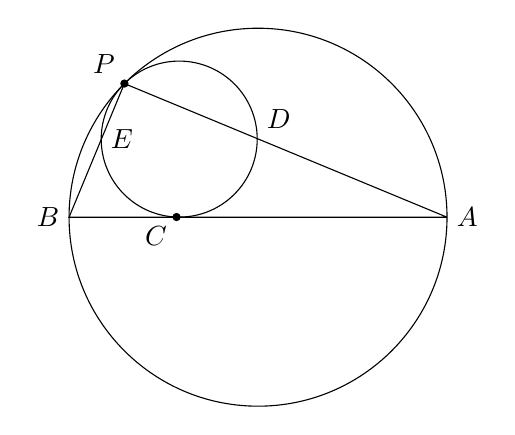
\begin{tikzpicture}[scale=0.3]
            \coordinate[label=right:$A$] (A) at (8, 0);
            \coordinate[label=left:$B$] (B) at (-8, 0);
            \coordinate[label=below left:$C$] (C) at (-3.45, 0.007);
            \coordinate[label=above right:$D$] (D) at (-0.035, 3.33);
            \coordinate[label=right:$E$] (E) at (-6.64, 3.29);
            \coordinate[label=above left:$P$] (P) at (-5.657, 5.657);
    
            \draw (0, 0) circle[radius=8];
            \draw (-3.337, 3.307) circle[radius=3.302];
            
            \draw (A) -- (B) -- (P) -- (A);
            \fill (P) circle[radius=5pt];
            \fill (C) circle[radius=5pt];
        \end{tikzpicture}
    \end{center}
\end{question}
\begin{center}
    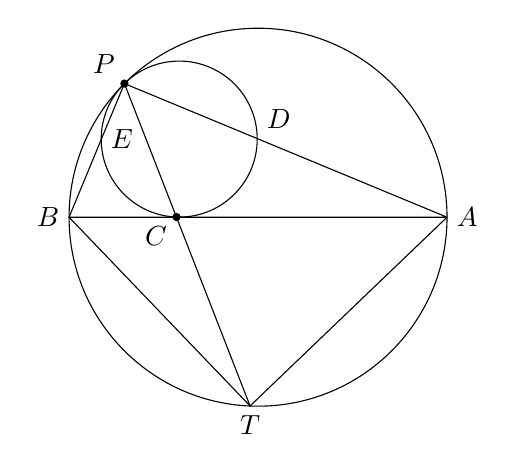
\begin{tikzpicture}[scale=0.3]
        \coordinate[label=right:$A$] (A) at (8, 0);
        \coordinate[label=left:$B$] (B) at (-8, 0);
        \coordinate[label=below left:$C$] (C) at (-3.45, 0.007);
        \coordinate[label=above right:$D$] (D) at (-0.035, 3.33);
        \coordinate[label=right:$E$] (E) at (-6.64, 3.29);
        \coordinate[label=above left:$P$] (P) at (-5.657, 5.657);
        \coordinate[label=below:$T$] (T) at (-0.337, -7.99);

        \draw (0, 0) circle[radius=8];
        \draw (-3.337, 3.307) circle[radius=3.302];
        
        \draw (A) -- (B) -- (P) -- (A);
        \fill (P) circle[radius=5pt];
        \fill (C) circle[radius=5pt];
        
        \draw (P) -- (T);
        \draw (B) -- (T) -- (A);

        \tkzMarkSegment[pos=.5,mark=|](B,T);
        \tkzMarkSegment[pos=.5,mark=|](T,A);
    \end{tikzpicture}
\end{center}
\begin{solution*}
    Consider the homothety $H$ at $P$ that maps the small circle to the big circle. Since $H(E) = B$ and $H(D) = A$, it follows that $\triangle PED$ and $\triangle PBA$ are similar. Let $H(C) = T$. Then $T$ is equidistant to $A$ and $B$, whence $PT$ bisects $\angle P$. Thus, by the angle bisector theorem, it follows that \[\frac{CA}{CB} = \frac{PA}{PB} = \frac{PD}{PE} = \frac{2}{3}.\] Since $CA + CB = 15$, we immediately have $CA = 9$.

    \begin{remark}
        This is an application of the \href{https://web.evanchen.cc/handouts/GeoSlang/GeoSlang.pdf}{Shooting Lemma}.
    \end{remark}
\end{solution*}

\clearpage
\begin{question}[160]\label{A::2024-S-1-18}
    On each face of a cube, an integer greater than 2 is written. Each vertex of the cube is the intersection of three unique faces, and each edge is the intersection of two unique faces. Assign to each vertex the product of the numbers written on the faces intersecting the vertex, and assign to each edge the product of the numbers written on the faces intersecting the edge. The sum of the numbers assigned to the eight vertices is equal to 2024. Find the maximum possible value of an edge.
\end{question}
\begin{solution*}
    Without loss of generality, let $f$, $b$, $l$, $r$, $u$, $d$ represent the numbers on the front, back, left, right, up, down faces of the cube respectively. We see that $(f + b)(l + r)(u + d) = 2024 = 2^3 \cdot 11 \cdot 23$. Since each face has an integer greater than 2, it follows that \[f + b = 8, \qquad l + r = 11, \qquad u + d = 23.\] Since we want to maximize only one edge, we take the edge joining $l$ and $u$, which is assigned \[(11 - \min r)(23 - \min d) = (11-3)(23-3) = 8 \cdot 20 = 160.\]
\end{solution*}

\begin{question}[72]\label{A::2024-S-1-19}
    Find the sum of the squares of each of the roots of the equation \[x^2 - 4\floor{x} - 12 = 0,\] where $\floor{x}$ denotes the greatest integer less than or equal to $x$.
\end{question}
\begin{solution*}
    Let $x = \floor{x} + \bc{x}$, where $\bc{x}$ denotes the fractional part of $x$. This turns the given equation into \[\floor{x}^2 - \floor{x}\bp{4 - 2\bc{x}} + \bp{\bc{x}^2 - 12} = 0.\] By the quadratic formula, we obtain \[\floor{x} = 2 - \bc{x} \pm 2\sqrt{4 - \bc{x}}.\] Since $\bc{x} \in [0, 1)$ and $\floor{x} \in \ZZ$, we see that $\floor{x} = -2, 5, 6$.

    \case{1}{$\floor{x} = -2$} The given equation reduces to $x^2 = 4$. Thus, $x = -2$ is a solution.

    \case{2}{$\floor{x} = 5$} The given equation reduces to $x^2 = 32$. Thus, $x = \sqrt{32}$ is a solution.

    \case{3}{$\floor{x} = 6$} The given equation reduces to $x^2 = 36$. Thus, $x = 6$ is a solution.

    Thus, the sum of the squares of the roots is $(-2)^2 + \sqrt{32}^2 + 6^2 = 72$.
\end{solution*}

\begin{question}[609]\label{A::2024-S-1-20}
    Calculate the remainder when $1901^{2024}$ is divided by 1216.
\end{question}
\begin{solution*}
    Notice that $1216 = 2^6 \cdot 19$. We can hence use the Chinese remainder theorem to tackle this problem. We obviously have $1901^{2024} \equiv 1 \pmod{19}$. We now calculate $1901^{2024} \pmod{64}$. Note that $1901 \equiv 45 \pmod{64}$. Additionally, since $\varphi(64) = 32$ and $2024 \equiv 8 \pmod{32}$, by Euler's theorem we immediately get \[1901^{2024} \equiv 45^8 \equiv 19^8 \equiv 561^4 \equiv 23^4 \equiv 529^2 \equiv 17^2 \equiv 289 \equiv 33  \pmod{64}.\] Let $n$ be the desired remainder. We hence have the following system of congruences: \[n \equiv 1 \pmod{19}, \qquad n \equiv 33 \pmod{64}.\] From the second congruence, we know $n = 33 + 64m$ for some integer $m$. Substituting this into the first congruence gives \[33 + 64m \equiv 1 \pmod{19} \implies 7m = 6 \pmod{19}.\] Note that the multiplicative inverse of 7 modulo 19 is 11 (since $11 \cdot 7 \equiv 1 \pmod{19}$). Hence, $m \equiv 6 \cdot 11 \equiv 9 \pmod{19}$. We thus get $m = 9 + 19k$ for some integer $k$. Substituting this back into the definition of $n$, we get \[n = 33 + 64(9 + 19k) = 609 + 64 \cdot 19k.\] Hence, the desired remainder is 609.
\end{solution*}

\begin{question}[521]\label{A::2024-S-1-21}
    Let $P(x) = a_0 + a_1 x + a_2 x^2 + \cdots + a_n x^n$ be a polynomial with non-negative integer coefficients satisfying $0 \leq a_i \leq 17$ for all $i$. If $P(18) = 367616$, find the value of $P(3)$.
\end{question}
\begin{solution*}
    Observe that the coefficients correspond to the digits of 367616 in base 18. Indeed, we see that \[367616 = 2 \cdot 18^0 + 11 \cdot 18^1 + 9 \cdot 18^3 + 3 \cdot 18^4.\] Hence, \[P(x) = 2 + 11x + 9x^3 + 3x^4,\] whence $P(3) = 521$.
\end{solution*}

\begin{question}[129]\label{A::2024-S-1-22}
    Evaluate the sum \[\frac{2}{1 + \tan{\frac{\pi}{260}}} + \frac{2}{1 + \tan{\frac{2\pi}{260}}} + \frac{2}{1 + \tan{\frac{3\pi}{260}}} + \cdots + \frac{2}{1 + \tan{\frac{129\pi}{260}}}.\]
\end{question}
\begin{solution*}
    Observe that we can pair each term with a corresponding term at the opposite end (except for the middle term): \[\sum_{k = 1}^{129} \frac{2}{1 + \tan{\frac{k\pi}{260}}} = 2\sum_{k = 1}^{64} \bs{\frac{1}{1 + \tan{\frac{k\pi}{260}}} + \frac{1}{1 + \tan{\frac\pi2 - \frac{k\pi}{260}}}} + \frac{2}{1 + \tan{\frac{65\pi}{260}}}.\] Since $\tan{\frac\pi2 - x} = \cot x$, we see that \[\sum_{k = 1}^{64} \bs{\frac{1}{1 + \tan{\frac{k\pi}{260}}} + \frac{1}{1 + \cot{\frac{k\pi}{260}}}} = \sum_{k = 1}^{64} \frac{1 + \cot{\frac{k\pi}{260}} + \tan{\frac{k\pi}{260}} + 1}{1 + \cot{\frac{k\pi}{260}} + \tan{\frac{k\pi}{260}} + 1} = 64.\] Thus, \[\sum_{k = 1}^{129} \frac{2}{1 + \tan{\frac{k\pi}{260}}} = 2 \cdot 64 + \frac{2}{1 + \tan{\frac{65\pi}{260}}} = 129.\]
\end{solution*}

\begin{question}[21]\label{A::2024-S-1-23}
    An equilateral triangle $ABC$ is inscribed in a circle and $P$ is a point on the minor arc $BC$. Point $D$ is the intersection of $AP$ and $BC$.

    \begin{center}
        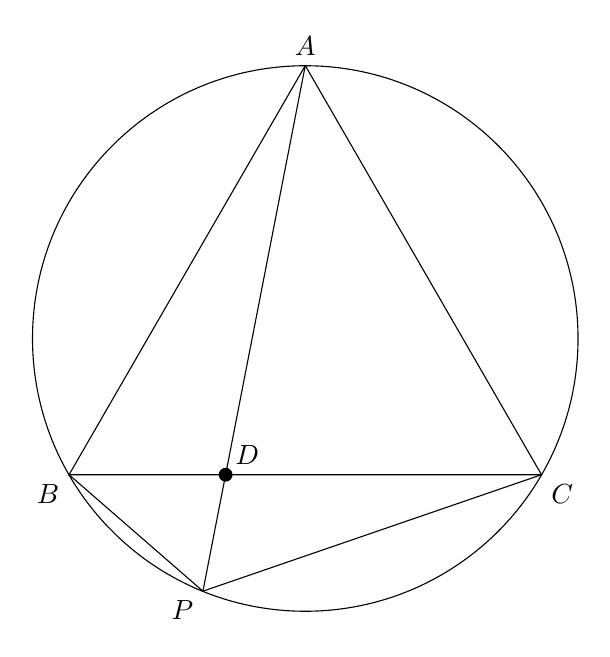
\begin{tikzpicture}
            \coordinate[label=above:$A$] (A) at (0, 5.196);
            \coordinate[label=below left:$B$] (B) at (-3, 0);
            \coordinate[label=below right:$C$] (C) at (3, 0);
            \coordinate[label=above right:$D$] (D) at (-1.011,0);
            \coordinate[label=below left:$P$] (P) at (-1.3, -1.479);
    
            \draw (A) -- (B) -- (C) -- (A);

            \draw (B) -- (P) -- (C);

            \draw (A) -- (P);
            \fill (D) circle[radius=2.5pt];
    
            \draw (0, 1.73) circle[radius=3.464];
        \end{tikzpicture}
    \end{center}

    \noindent Suppose that $BP = 5$, $CP = 20$. Find the length of $AD$.
\end{question}
\begin{solution*}
    Let $s$ be the side length of the equilateral triangle. By Ptolemy's theorem, we know that \[BP \cdot AC + BA \cdot CP = BC \cdot AP \implies AD + DP = 25.\] Notice that $\triangle BDP$ is similar to $\triangle ADC$. Hence, \[\frac{DP}{BP} = \frac{CD}{CA} \implies CD = \frac{s \cdot DP}{5}, \qquad \frac{BD}{BP} = \frac{AD}{AC} \implies BD = \frac{5 AD}{s}.\] Likewise, $\triangle ADB$ is similar to $\triangle CDP$, whence \[\frac{CD}{CP} = \frac{AD}{AB} \implies CD = \frac{20 AD}{s}.\] We thus see that \[s = BD + DC = \frac{25 AD}{s} \implies s^2 = 25 AD,\] and \[CD = \frac{s \cdot DP}{5} = \frac{20 AD}{s} \implies DP = \frac{100 AD}{s^2} = \frac{100 AD}{25 AD} = 4.\] Thus, $AD = 25 - DP = 21$.
\end{solution*}

\begin{question}[94]\label{A::2024-S-1-24}
    Find the number of positive integers $x < 9000$ such that $x^3 + 95$ is divisible by 96.
\end{question}
\begin{solution*}
    We are given that \[x^3 + 95 \equiv 0 \pmod{96} \implies x^3  - 1 \equiv 0 \pmod{96}.\] Since $96 = 2^5 \cdot 3$, we have $x^3 - 1 \equiv 0$ modulo 3 and 32. Note that $x^3 - 1 \equiv 0 \pmod{3}$ has a unique solution $x \equiv 1 \pmod{3}$. Furthermore, by repeatedly applying Hensel's lemma, it is not too hard to see that $x \equiv 1 \pmod{32}$ is the unique solution to $x^3 - 1 \equiv 0 \pmod{32}$. It thus follows by the Chinese remainder theorem that $x \equiv 1 \pmod{96}$ is the only solution to $x^3 - 1 \equiv 0 \pmod{96}$. That is, we have $x = 1 + 96k$ for integers $k \geq 0$. Since $x < 9000$, we have $k < \frac{8999}{96} \approx 93.7$. Thus, $k \in \bc{0, 1, \ldots, 93}$, whence there are 94 possibilities for $x$.
\end{solution*}

\begin{question}[26]\label{A::2024-S-1-25}
    A scalene triangle $\triangle ABC$ has sides $AB = 7$, $AC = 12$ and $BC = 13$. Write $\tan \frac{A-B}{2} \tan \frac{C}{2}$ as a fraction $\frac{m}{n}$ in its lowest form and find $m + n$.

    \begin{center}
        \begin{tikzpicture}[scale=0.5]
            \coordinate[label=above:$A$] (A) at (2.85, 6.40);
            \coordinate[label=below right:$B$] (B) at (13, 0);
            \coordinate[label=below left:$C$] (C) at (0, 0);
    
            \draw (A) -- (B) -- (C) -- (A);
    
            \node[anchor=south west] at ($(A)!0.5!(B)$) {7};
            \node[anchor=north] at ($(B)!0.5!(C)$) {13};
            \node[anchor=south east] at ($(C)!0.5!(A)$) {12};
        \end{tikzpicture}
    \end{center}
\end{question}
\begin{solution*}
    Observe that $\frac{C}{2} = 90\deg - \frac{A + B}{2}$. Hence, \[\tan \frac{C}{2} = \tan{90\deg - \frac{A + B}{2}} = \cot \frac{A + B}{2}.\] The desired product is hence \[\tan \frac{A-B}{2} \tan \frac{C}{2} = \frac{\sin \frac{A-B}{2} \cos \frac{A+B}{2}}{\cos \frac{A-B}{2} \sin \frac{A+B}{2}} = \frac{2\sin \frac{A-B}{2} \cos \frac{A+B}{2}}{2\cos \frac{A-B}{2} \sin \frac{A+B}{2}}.\] By the product-to-sum identities, this immediately simplifies to \[\frac{2\sin \frac{A-B}{2} \cos \frac{A+B}{2}}{2\cos \frac{A-B}{2} \sin \frac{A+B}{2}} = \frac{\sin A - \sin B}{\sin A + \sin B}.\] By the sine rule, we have $\sin A = \frac{a}{b} \sin B$. Thus, \[\frac{\sin A - \sin B}{\sin A + \sin B} = \frac{\frac{a}{b} - 1}{\frac{a}{b} + 1} = \frac{a - b}{a + b} = \frac{13 - 12}{13 + 12} = \frac{1}{25}.\] Hence, $m + n = 26$.
\end{solution*}